\section{Signalklassen}{2}

Signale lassen sich vielfach klassieren, beispielsweise folgendermassen:

\begin{center}
    \begin{tabular}{lcl}
        \toprule
        kontinuierlich          & \textlrarrow\ & zeitdiskret               \\
        \midrule
        analog                  & \textlrarrow\ & digital                   \\
        \midrule
        reell                   & \textlrarrow\ & komplex                   \\
        \midrule
        eindimensional (SISO)   & \textlrarrow\ & mehrdimensional (MIMO)    \\
        \midrule
        deterministisch         & \textlrarrow\ & stochstisch               \\
        \midrule
        periodisch              & \textlrarrow\ & nicht periodisch          \\
        \bottomrule
    \end{tabular}
\end{center}


\subsection{Energie- und Leistungssignale}{3}

\begin{center}
    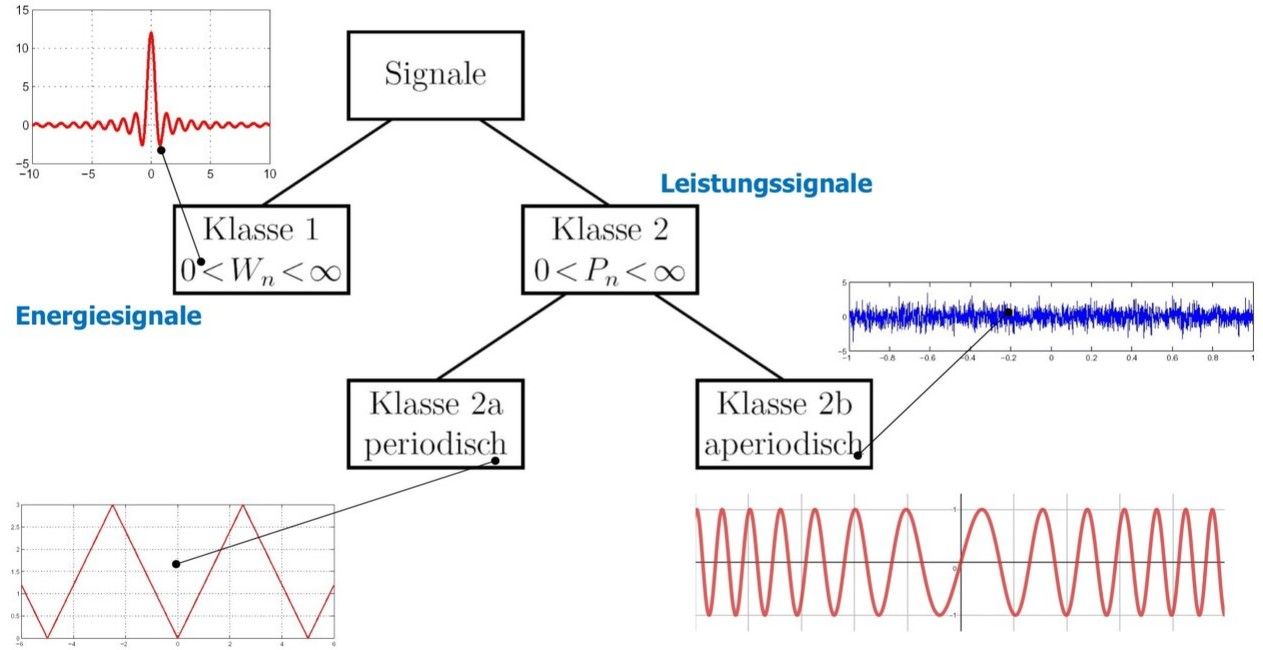
\includegraphics[width=0.85\columnwidth]{images/klassierung_signale_2.jpg}
\end{center}

Signale der Klasse 2 sind näherungsweise zeitlich begrenzte Signale  $(W_n = \infty)$ 

\vspace{0.2cm}
Alle beschränkten Signale endlicher Dauer, die auf einem endlichen Zeitintervall von Null verschieden sind, 
sind stets Energiesignale und gehören zur Klasse 1.


\subsubsection{Normierte Signalenergie $\bm{W_n}$ / Normierte Signalleistung $\bm{P_n}$}

\begin{minipage}{0.48\columnwidth}
    $$ \boxed{ W_n = \lim\limits_{T \to \infty} \int\limits_{-T/2}^{T/2} \vert f(t) \vert ^2 \, \diff t } $$
\end{minipage}
\hfill
\begin{minipage}{0.48\columnwidth}
    $$ \boxed{ P_n = \lim\limits_{T \to \infty} \frac{1}{T} \int\limits_{-T/2}^{T/2} \vert f(t) \vert ^2 \, \diff t } $$ 
\end{minipage}

\vspace{0.2cm}

\textbf{Hinweis:} Wenn $W_n$ endlich ist, dann ist $P_n = 0$

